\documentclass{article}
\usepackage{graphicx} % Required for inserting images
\usepackage{amsmath}

\title{Séries temporais}
\author{Mariana Fernandes Rocha}
\date{September 2025}

\begin{document}


\begin{titlepage}
    \begin{center}

        \vspace{1cm}
        \begin{minipage}{0.45\textwidth}
            \centering
            
\includegraphics[width=1.2\textwidth]{images/logo_fgv.png}    
        \end{minipage}
        \vspace{2cm}

        \rule{1\textwidth}{0.4pt} \\ % Linha horizontal personalizada
        \vspace{0.2cm}
        {\Huge \textbf{Análise de Séries Temporais}} \\
        \vspace{0.2cm}
        \vspace{0.5cm}\\
        {\Large \textbf{A1 - Séries Temporais}}\\
        \rule{1\textwidth}{0.4pt} % Linha horizontal personalizada


        \vspace{0.5cm}
        {\Large \textbf{FGV EMAp}} \\
        \vspace{2cm}
        
        

        
        
        % % Unidade e curso
        % {\Large \textbf{FGV EMAp}}\\[2cm]
        
        % Autores
        {\large 
            \textbf{Ana Júlia Amaro Pereira Rocha} \\ 
            \textbf{Henrique Borges Carvalho} \\
            \textbf{Maria Eduarda Mesquita Magalhães}\\
            \textbf{Mariana Fernandes Rocha} \\
            \textbf{Paula Eduarda de Lima}}\\[1.5cm]
        
        % Informações adicionais
        {\large 
            Ciência de Dados e Inteligência Artificial \\ 
            6º Período}\\[2cm]
        
         % Data
        \vfill
        {\large Rio de Janeiro, 2025}

        
    \end{center}
\end{titlepage}

\section{Discussão sobre métricas e métodos de avaliação}

Para previsões pontuais temos dois grupos de métricas e avaliação:
\begin{itemize}
    \item Métricas percentuais;
    \item Métricas envolvendo escala: escaladas e dependentes de escala;
\end{itemize}
Métricas percentuais são adequadas para cenários em que os valores devem ter ordem de grandeza clara e consistente, e mais importante assumir valores distantes de zero, causando distorções quando $y_t \to 0, \dfrac{e_t}{y_t} \to \infty$.

 Primeiramente, mais um terço dos dados assume valores menores que 1, o intervalo que mais sofre com a distorção. Outro ponto, o intervalo dos dados $[0.14 , 16.59]$ não representa uma escala de grandeza bem compreendida, e com esses argumentos concluímos que métricas percentuais não são convenientes para nossos dados.

\begin{figure}[h]
    \centering
    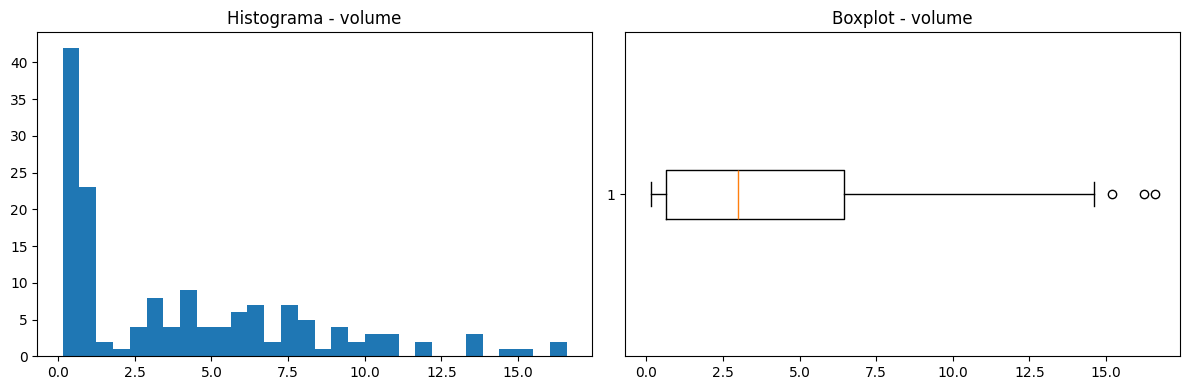
\includegraphics[width=0.75\linewidth]{images/histogram.png}
    \caption{Histograma e distribuição dos valores}
    % \label{fig:placeholder}
\end{figure}

Métricas escaladas e métricas dependentes de escala são parecidas, mas não iguais. As métricas escaladas ajustam o erro pela magnitude dos dados, erros sem medida e mais comparáveis entre problemas distintos. Já as métricas dependentes mantêm o erro na mesma unidade da variável alvo.

No nosso experimento, utilizamos o mesmo conjunto de dados para testar múltiplos modelos, assim optamos por métricas escaladas. Elas facilitam a interpretação, especialmente por públicos leigos, e permitem comparações mais intuitivas, é mais claro dizer que o modelo 1 teve 10\% de melhora em relação ao modelo 2, do que comparar erros absolutos como 5 e 5,5 na variável "volume", cujas unidades não temos familiaridade.

Com isso em mente, vamos utilizar para previsões pontuais o MASE:

$$MASE = \dfrac{\text{MAE do modelo}}{\text{MAE do modelo de referência}}$$

Um exemplo numérico, o MAE do seu modelo foi 4.2 e  o MAE do modelo referência foi 6.0, então $MASE
=\frac{4.2}{6.0}= 0.7$. Isso significa que seu modelo erra 30\% menos do que a referência.

Embora o foco até aqui tenha sido a avaliação de previsões pontuais, também serão abordadas previsões distribucionais, o ponto mais importante dessa avaliação é incorporar a incerteza associada às estimativas.
Para isso, derivamos distribuições preditivas a partir da análise dos resíduos dos modelos, assumindo que seguem uma distribuição normal. Essa abordagem possibilita a construção de intervalos de predição e a utilização de métricas específicas para avaliação probabilística, como o CRPS e o Winkler Score.
\begin{itemize}
    \item \textbf{CRPS}: compara a função de distribuição acumulada (CDF) da previsão com o valor observado. Matematicamente, ele mede a área entre a CDF predita (F(x)) e a CDF empírica do valor observado.
    $$CRPS(F, y_t) = \int_{-\infty}^{\infty}(F(x)- \mathbb{1}(x \geq y_t))^2 dx $$
    \item \textbf{Winkler Score}: qualidade dos intervalos de predição gerados por um modelo, penaliza tanto a não cobertura do valor real quanto intervalos excessivamente amplos.

    $$
W_{\alpha, t} = 
\begin{cases}
(u_{\alpha, t} - l_{\alpha, t}) + \frac{2}{\alpha} (l_{\alpha, t} - y_t), & \text{se } y_t < l_{\alpha, t} \\
(u_{\alpha, t} - l_{\alpha, t}), & \text{se } l_{\alpha, t} \leq y_t \leq u_{\alpha, t} \\
(u_{\alpha, t} - l_{\alpha, t}) + \frac{2}{\alpha} (y_t - u_{\alpha, t}), & \text{se } y_t > u_{\alpha, t}
\end{cases}
    $$
\end{itemize}


\section{Discussão sobre a necessidade de transformação de variáveis}


\section{Discussão sobre a necessidade de decomposição entre tendência e sazonalidade}

\section{Análises de resíduos e ajuste dos modelos}
\section{Modelos baselines}

Modelos baseline são abordagens de previsão simples que servem como um ponto de referência para avaliar o desempenho de modelos mais complexos. A sua principal função é estabelecer um limiar de performance: se um modelo sofisticado não conseguir superar um baseline simples, isso sugere que o modelo mais complexo não está capturando bem os padrões da série ou que a série é inerentemente difícil de prever. Para este trabalho, foram implementados cinco modelos baseline, cujos resultados foram comparados utilizando as métricas MAE, RMSE e MAPE.

\subsection{Mean Method}
Este é o baseline mais simples, onde a previsão para qualquer período futuro é a média de todos os valores observados no conjunto de treino.
$$ \hat{y}_{T+h|T} = \bar{y} = \frac{1}{T}\sum_{t=1}^{T}y_t $$

\subsection{Naive Method}
Neste método, a previsão para o próximo período é simplesmente o último valor observado.
$$ \hat{y}_{T+h|T} = y_T $$

\subsection{Seasonal Naive}
Uma variação do Naive Method, útil para séries com forte sazonalidade. Ele prevê o valor futuro utilizando a observação do mesmo período no ciclo sazonal anterior. Utilizamos dados semanis considerando sazonalidade anual, o período é $m=52$.
$$ \hat{y}_{T+h|T} = y_{T+h-m} $$

\subsection{Drift Method}
Este método é uma extensão do Naive e é adequado para séries com tendência. Ele extrapola uma linha traçada entre a primeira e a última observação do conjunto de treino. A previsão incorpora uma "inclinação" (drift) média.
$$ \hat{y}_{T+h|T} = y_T + h \left( \frac{y_T - y_1}{T-1} \right) $$

\subsection{Média Móvel}
A previsão é calculada como a média dos últimos $K$ valores observados no conjunto de treino. Este método suaviza flutuações de curto prazo. Para este estudo, foi utilizado $K=4$.
$$ \hat{y}_{T+h|T} = \frac{1}{K}\sum_{t=T-K+1}^{T}y_t $$

\subsection{Resultados e Análise}
Os modelos foram treinados com os primeiros 120 pontos da série e avaliados nos 30 pontos subsequentes. Os resultados obtidos para as métricas de erro no conjunto de teste estão consolidados na Tabela 1.

\begin{table}[h]
    \centering
    \begin{tabular}{|l|c|c|c|}
        \hline
        \textbf{Modelo} & \textbf{MAE} & \textbf{RMSE} & \textbf{MAPE (\%)} \\
        \hline
        Drift & 3.9666 & 4.6585 & 34.40 \\
        Seasonal Naive & 4.7593 & 5.4027 & 44.01 \\
        Naive & 4.6803 & 5.4411 & 40.79 \\
        Média móvel (k=4) & 5.0153 & 5.7318 & 44.20 \\
        Mean & 7.9639 & 8.4335 & 74.25 \\
        \hline
    \end{tabular}
    \caption{Resultados dos Modelos Baseline no Conjunto de Teste.}
    \label{tab:baseline_results}
\end{table}

Analisando a Tabela \ref{tab:baseline_results}, o \textbf{Drift Mathod} apresentou o melhor desempenho em todas as métricas, com um RMSE de 4.6585. Isso sugere que a série possui uma componente de tendência linear que é capturada de forma eficaz por este método. Os modelos Naive e Seasonal Naive tiveram performances intermediárias e muito similares, indicando que tanto a dependência do último ponto quanto a sazonalidade anual são características relevantes, mas secundárias à tendência geral. O Mean Method foi o que obteve o pior resultado, o que era esperado para uma série não estacionária com tendência.

O desempenho do modelo de Drift estabelece, portanto, o principal benchmark a ser superado pelos modelos mais complexos que serão analisados nas próximas seções.

\section{Modelos de regressão linear múltipla}

\end{document}
